
\subsection{Waste Form Degradation Rate}


The sensitivity of peak dose rate to the waste form degradation rate was 
determined with respect to varying inventories of waste.

The sensitivity of repository performance to waste form degradation rate was
expected to vary according to the waste inventory. For cases in which the dominant dose contributing 
radionuclides have half-lives much shorter than the expected waste form lifetime, 
the waste form degradation rate is not expected to have an effect. So too, for 
cases in which the primary barrier to release, the slow diffusive pathway, 
dominates overall repository performance, the waste form engineered barrier was
expected to have a negligible effect on repository performance in comparison.

In the case of a clay repository, the effect of the long time scale of the 
diffusive release pathway was to dampen the potential effect of high waste form 
degradation rates. 

\subsubsection{Parametric Range}

These runs varied the waste form degradation rate and the waste inventory mass 
factor.  There were forty runs corresponding to eight values of the waste form degradation 
rate and five values of the mass factor.

The waste form degradation rate was varied over the eight magnitudes 
between $10^{-9}$ and $10^{-2} [1/yr]$. The inventory mass factor was varied 
over the five magnitudes between $0.001$ and $10.0 [-]$. 

\subsubsection{Results}

These results show two regimes. In the first regime, the mean of the peak annual 
dose rates is directly proportional to both the mass factor and the fractional 
waste form degradation rate. For some radionuclides, attenuation occurs for high 
values of both parameters as the release of radionuclides is limited by 
dispersion parameters. This phenomenon can be seen in the figures below in which 
transition between regimes for higher degradation rates happens at lower mass 
factors than transition between regimes for lower degradation rates. 

Safety indicators for post closure repository performance have been developed by 
the \gls{UFD} campaign which utilize the inventory multiplier that was varied in 
this study \cite{nutt_generic_2009}. These indicators are normalized by a 
normalization factor (100 mrem/yr) recommended by the \gls{IAEA} as the limit to 
``relevant critical members of the public'' \cite{iaea_international_1996}. The functional form for 
this safety indicator for a single waste category, \gls{HLW}, is just 

\begin{align}
SI_{G} &= \left(\frac{\sum_{i=1}^{N}D_{G,i}(I_i, F_{d})}{100mrem/yr}\right)[GWe/yr].
\label{indicator}
\intertext{where}
SI_{G} &= \mbox{Safety indicator for disposal in media type G}[GWe/yr]\nonumber\\
N &= \mbox{Number of key radionuclides considered in this indicator}\nonumber\\
D_{G,i} &= \mbox{Peak dose rate from isotope i in media type G}[mrem/yr]\nonumber\\
F_{d} &= \mbox{Fractional waste form degradation rate}[1/yr].\nonumber
\end{align}

Tables \ref{tab:WFDegIndicatorsTcICsSeCl}, 
\ref{tab:WFDegIndicatorsPdSnZrNb}, and 
\ref{tab:WFDegIndicatorsActinides} report the safety indicators for 
various independent isotopes and, where applicable, their daughters. 

\begin{table}[h!]
\centering
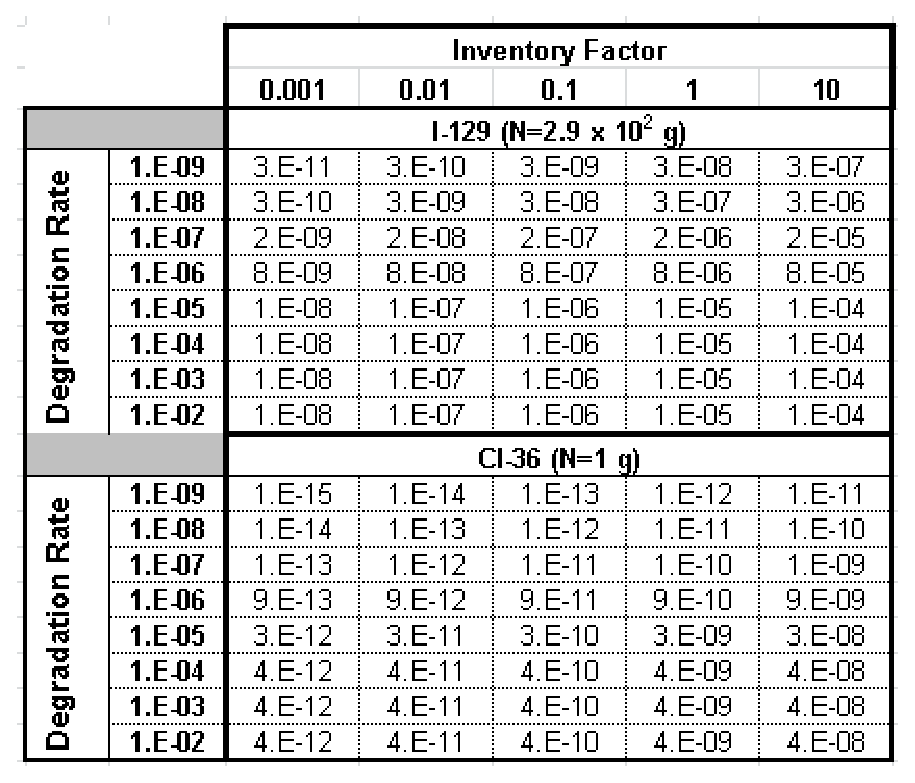
\includegraphics[width=0.5\textwidth]{./chapters/nuclide_sensitivity/clay/WFDegAndInv/IndicatorsSolNonSorbing.eps}
\caption{Safety indicators for soluble, non-sorbing nuclides.} 
\label{tab:WFDegIndicatorsTcICsSeCl}
\end{table}

\begin{table}[h!]
\centering
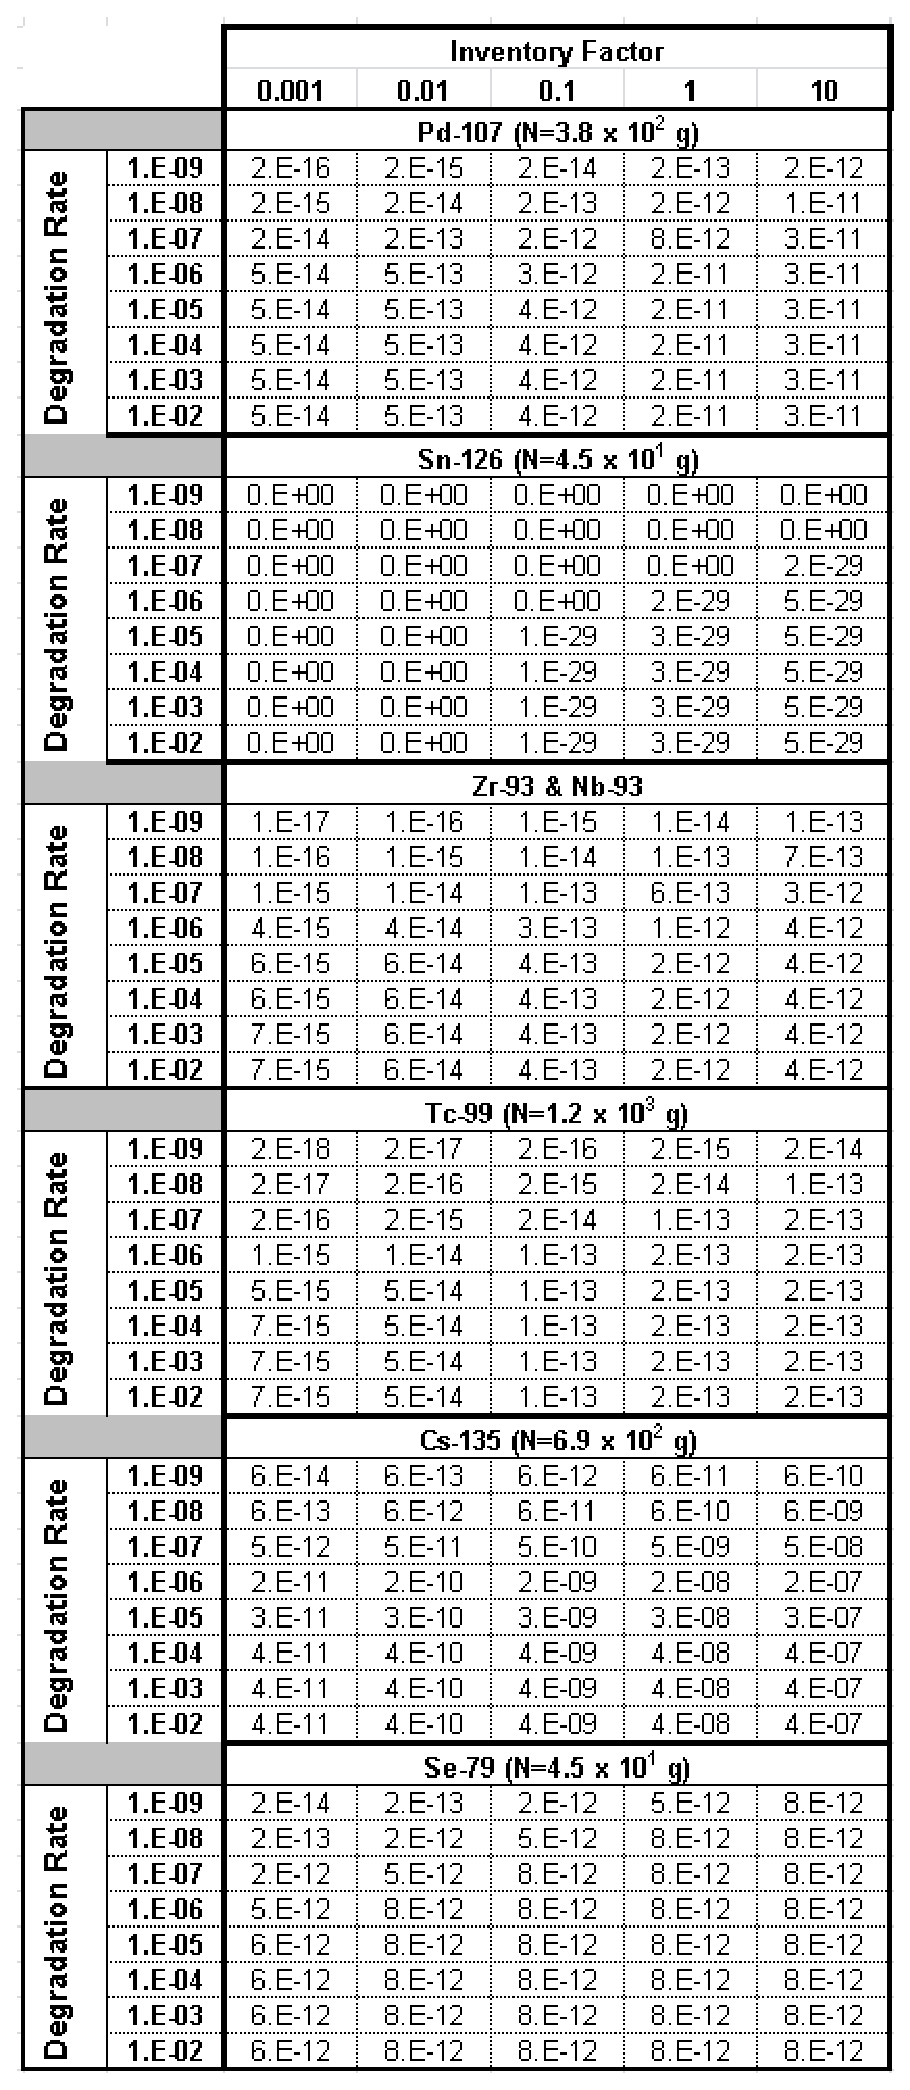
\includegraphics[width=0.5\textwidth]{./chapters/nuclide_sensitivity/clay/WFDegAndInv/IndicatorsSolLimSorbing.eps}
\caption{Safety indicators for solubility limited and sorbing nuclides.} 
\label{tab:WFDegIndicatorsPdSnZrNb}
\end{table}

\begin{table}[h!]
\centering
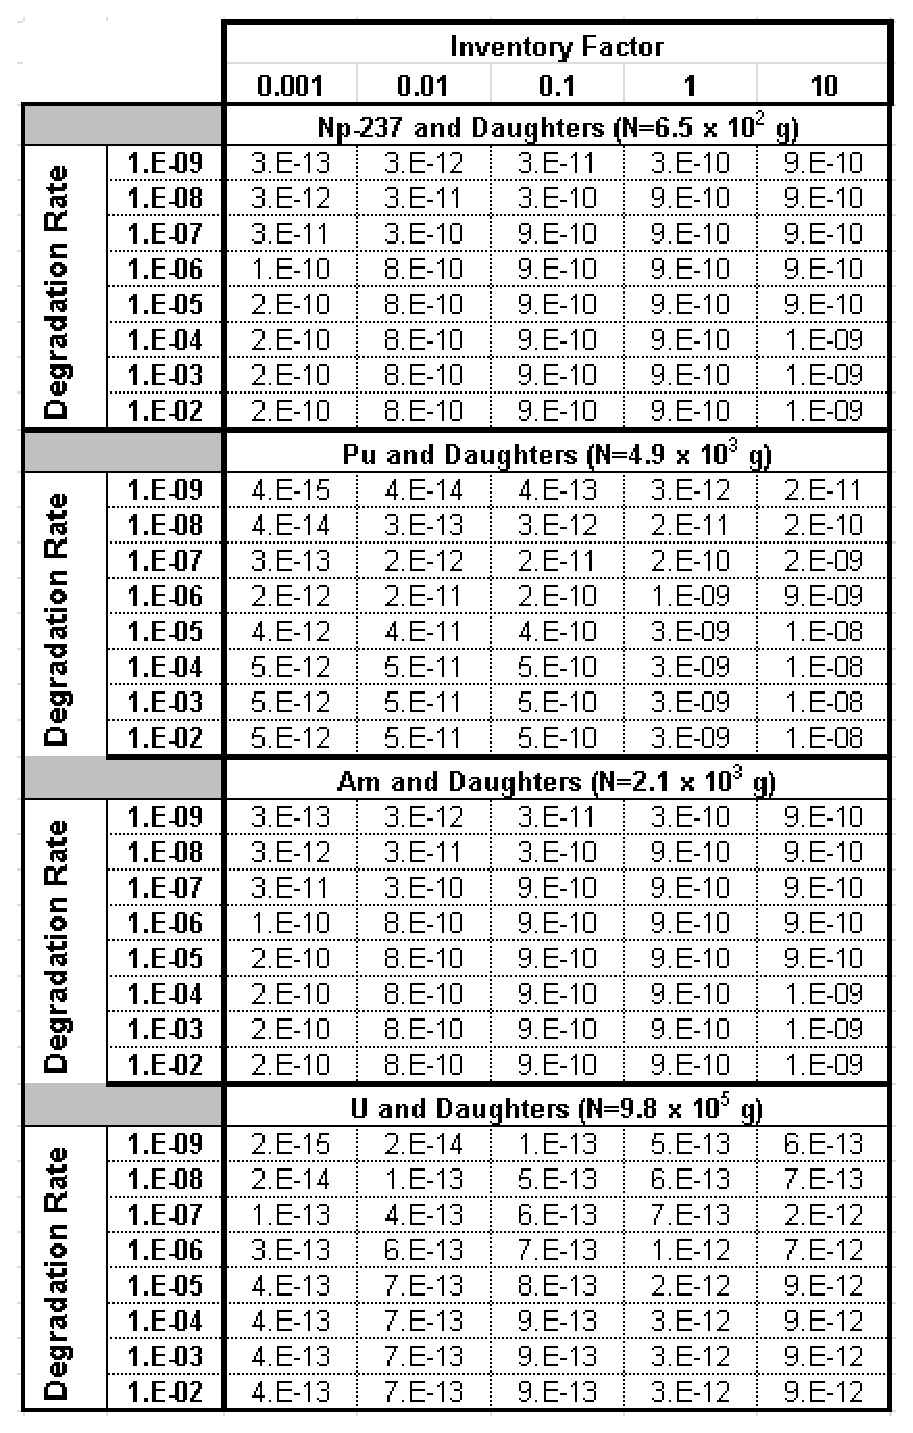
\includegraphics[width=0.5\textwidth]{./chapters/nuclide_sensitivity/clay/WFDegAndInv/IndicatorsActinides.eps}
\caption{Safety indicators for the actinides and their daughters.}
\label{tab:WFDegIndicatorsActinides}
\end{table}

\clearpage 
The peaks for highly soluble, non sorbing elements such as $I$ and $Cl$
are directly proportional to mass factor for most 
values of waste form degradation rates. This effect can be seen in Figures 
\ref{fig:WFDegI129}, \ref{fig:WFDegI129MF}, \ref{fig:WFDegCl36}, and 
\ref{fig:WFDegCl36MF}. 


Highly soluble and non-sorbing $^{129}I$ demonstrates a direct proportionality between dose rate and 
fractional degradation rate until a turnover where other natural system 
parameters dampen transport. Highly soluble and non-sorbing $^{129}I$ domonstrates a direct 
proportionality to the inventory multiplier.

\begin{figure}[ht!]
\begin{minipage}[b]{0.45\linewidth}
\centering
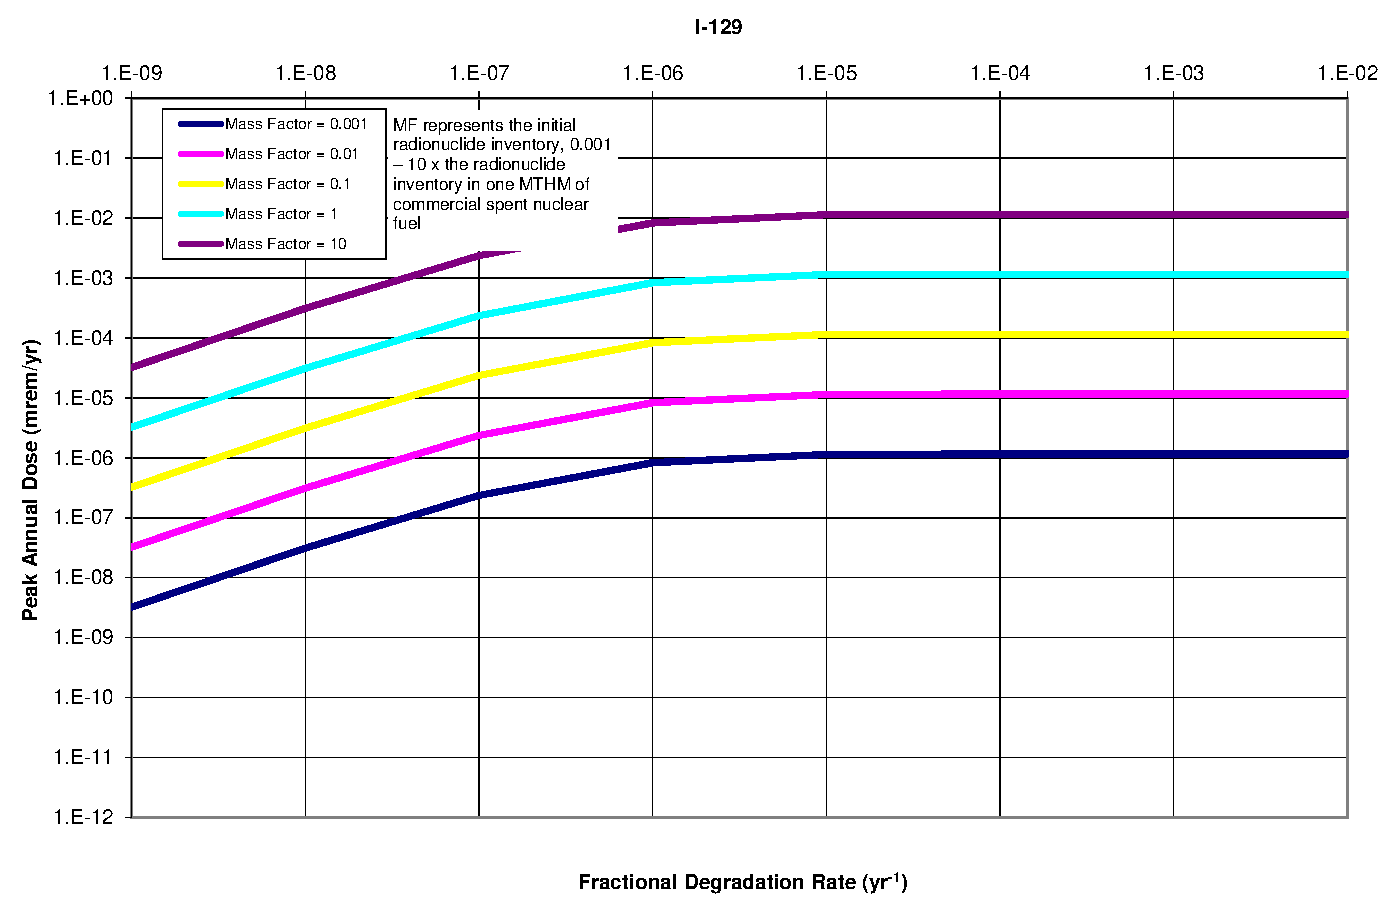
\includegraphics[width=\linewidth]{./chapters/nuclide_sensitivity/clay/WFDegAndInv/I-129.eps}
\caption{$^{129}I$ waste form degradation rate sensitivity.}
\label{fig:WFDegI129}

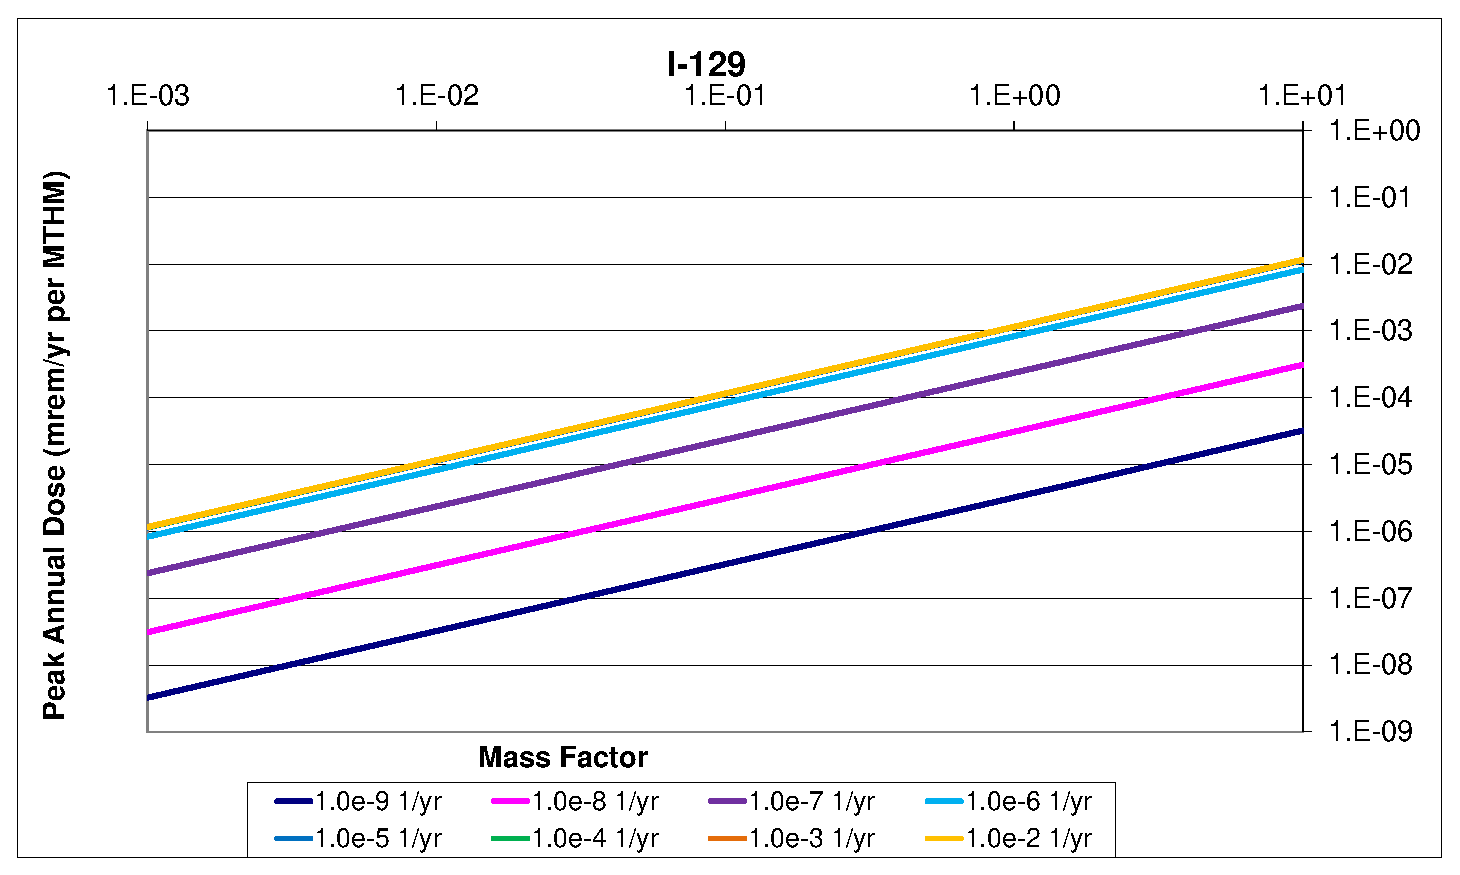
\includegraphics[width=\linewidth]{./chapters/nuclide_sensitivity/clay/WFDegAndInv/I-129-MF.eps}
\caption{$^{129}I$ inventory multiplier sensitivity.}
\label{fig:WFDegI129MF}

\end{minipage}
\hspace{0.05\linewidth}
\begin{minipage}[b]{0.45\linewidth}

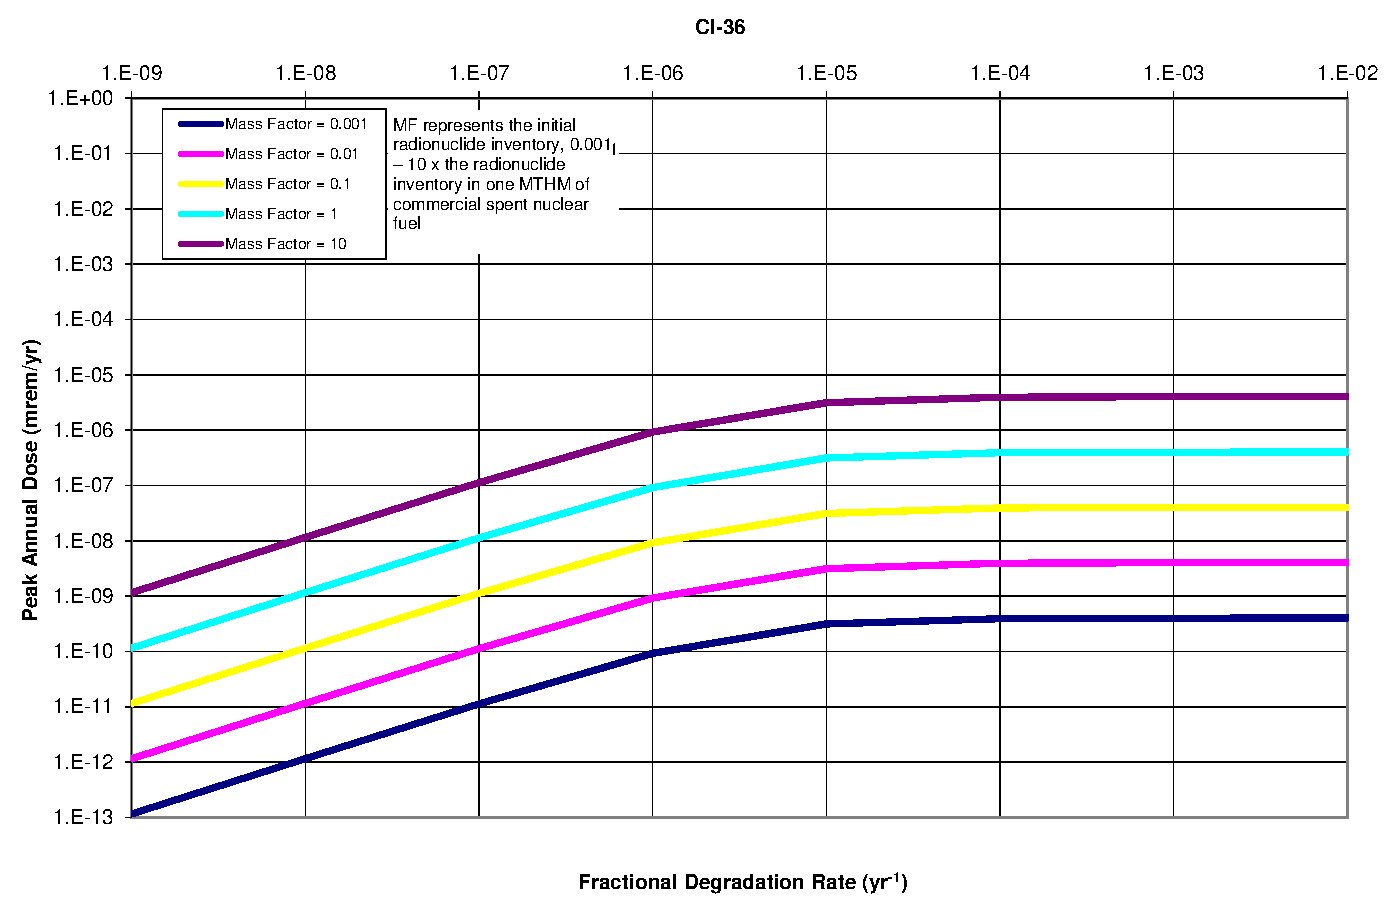
\includegraphics[width=\linewidth]{./chapters/nuclide_sensitivity/clay/WFDegAndInv/Cl-36.eps}
\caption{$^{36}Cl$ waste form degradation rate sensitivity.}
\label{fig:WFDegCl36}

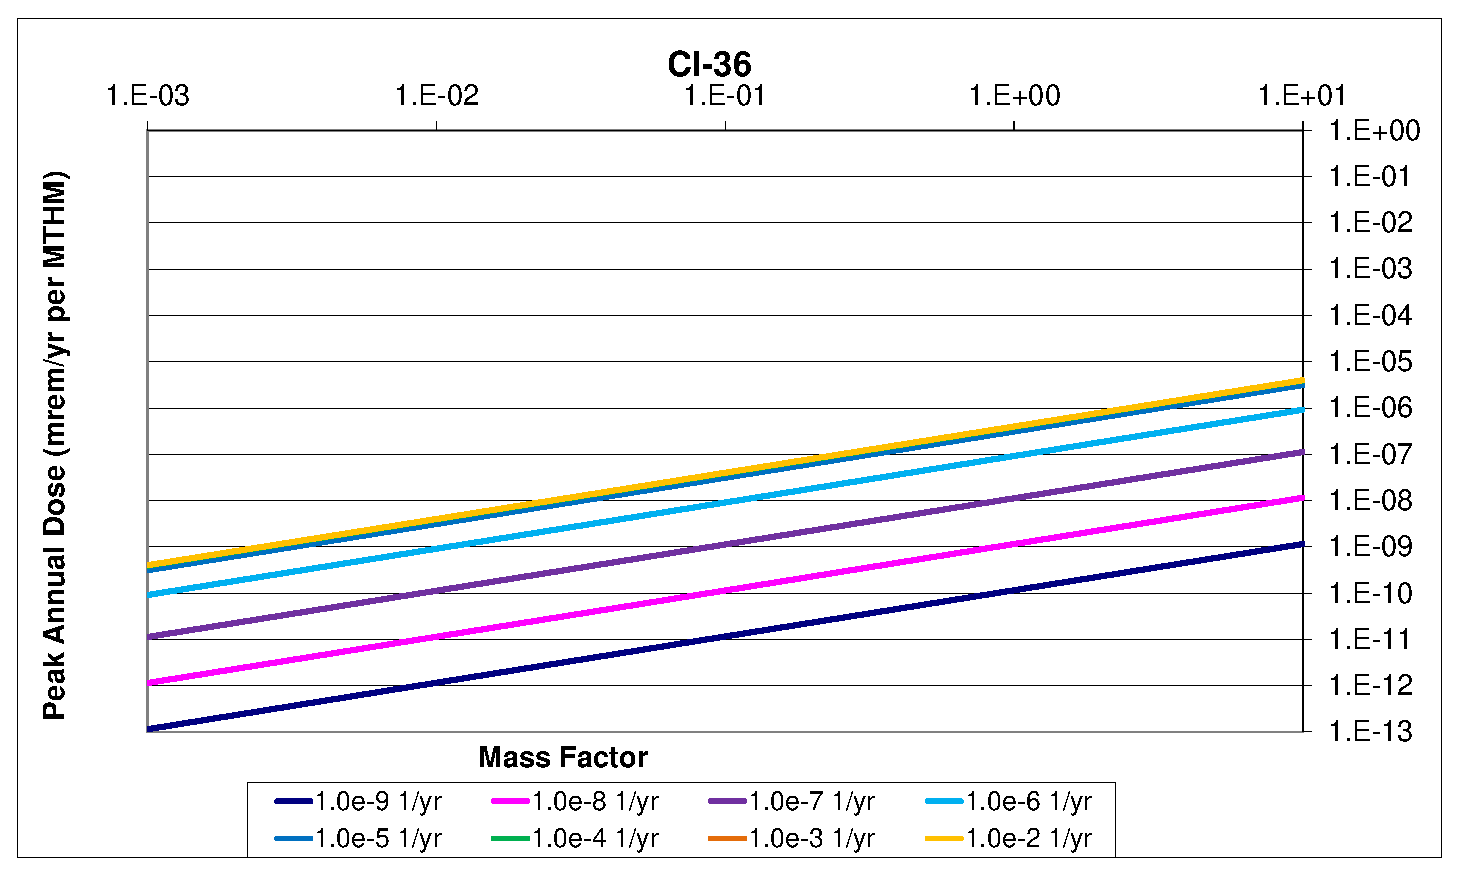
\includegraphics[width=\linewidth]{./chapters/nuclide_sensitivity/clay/WFDegAndInv/Cl-36-MF.eps}
\caption{$^{36}Cl$ inventory multiplier sensitivity.}
\label{fig:WFDegCl36MF}
\end{minipage}
\end{figure}
\clearpage

The peaks for solubility limited, sorbing elements such as $Tc$ and $Np$, on the 
other hand, have a more dramatic turnover.  For very high degradation rates, the 
dependence on mass factor starts to round off due to attenuation by solubility 
limits, as can be seen in Figures \ref{fig:WFDegNp237}, \ref{fig:WFDegNp237MF}, 
\ref{fig:WFDegTc99}, and \ref{fig:WFDegTc99MF}.

Solubility limited and sorbing $^{99}Tc$ demonstrates a direct proportionality 
to fractional degradation rate until attuation by its solubility limit and other 
natural system parameters.  

\begin{figure}[ht!]
\begin{minipage}[b]{0.45\linewidth}

\centering
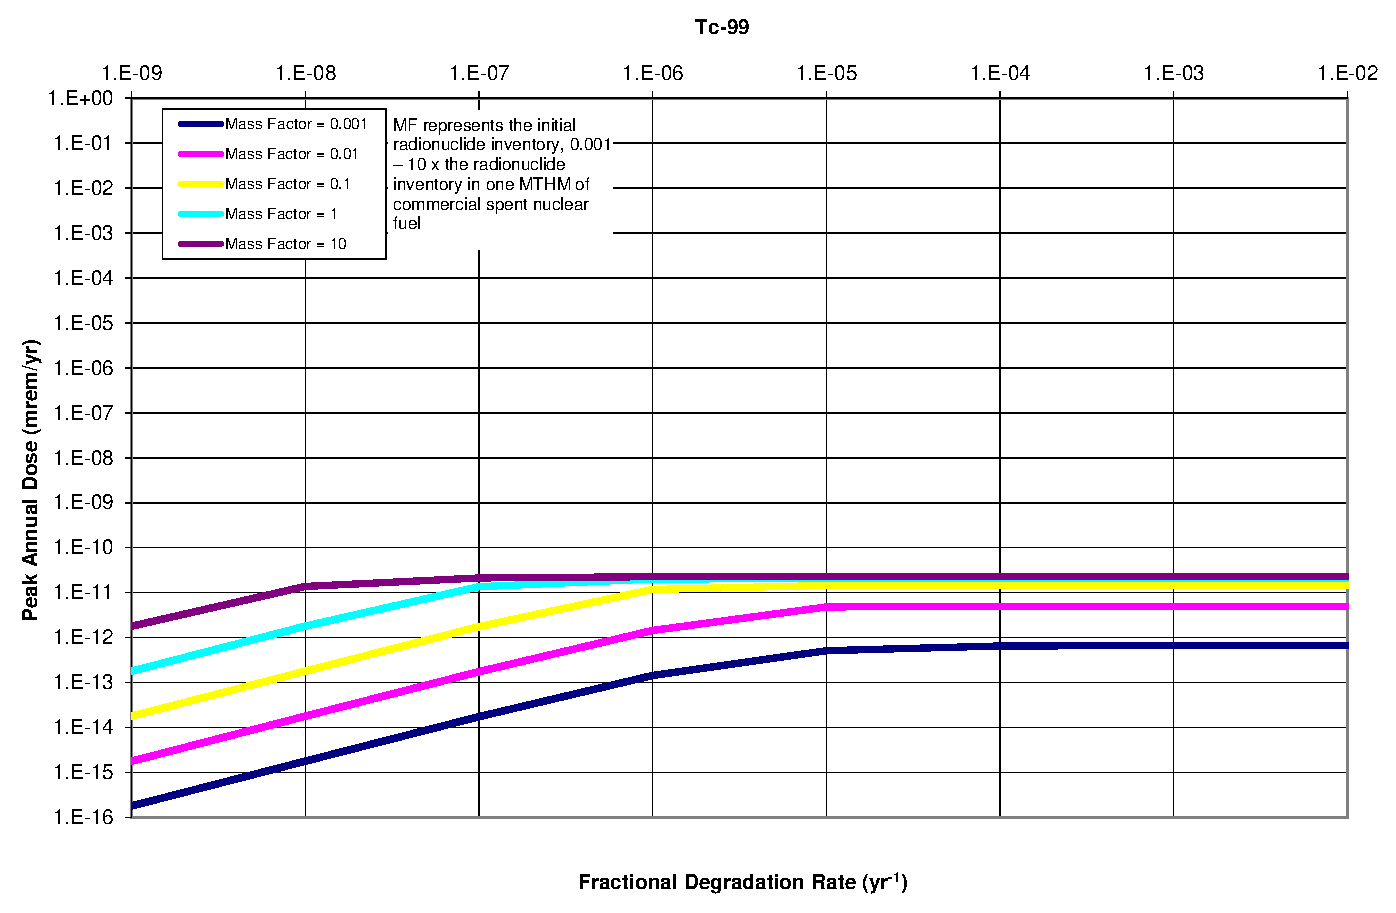
\includegraphics[width=\linewidth]{./chapters/nuclide_sensitivity/clay/WFDegAndInv/Tc-99.eps}
\caption{$^{99}Tc$ waste form degradation rate sensitivity.}
\label{fig:WFDegTc99}

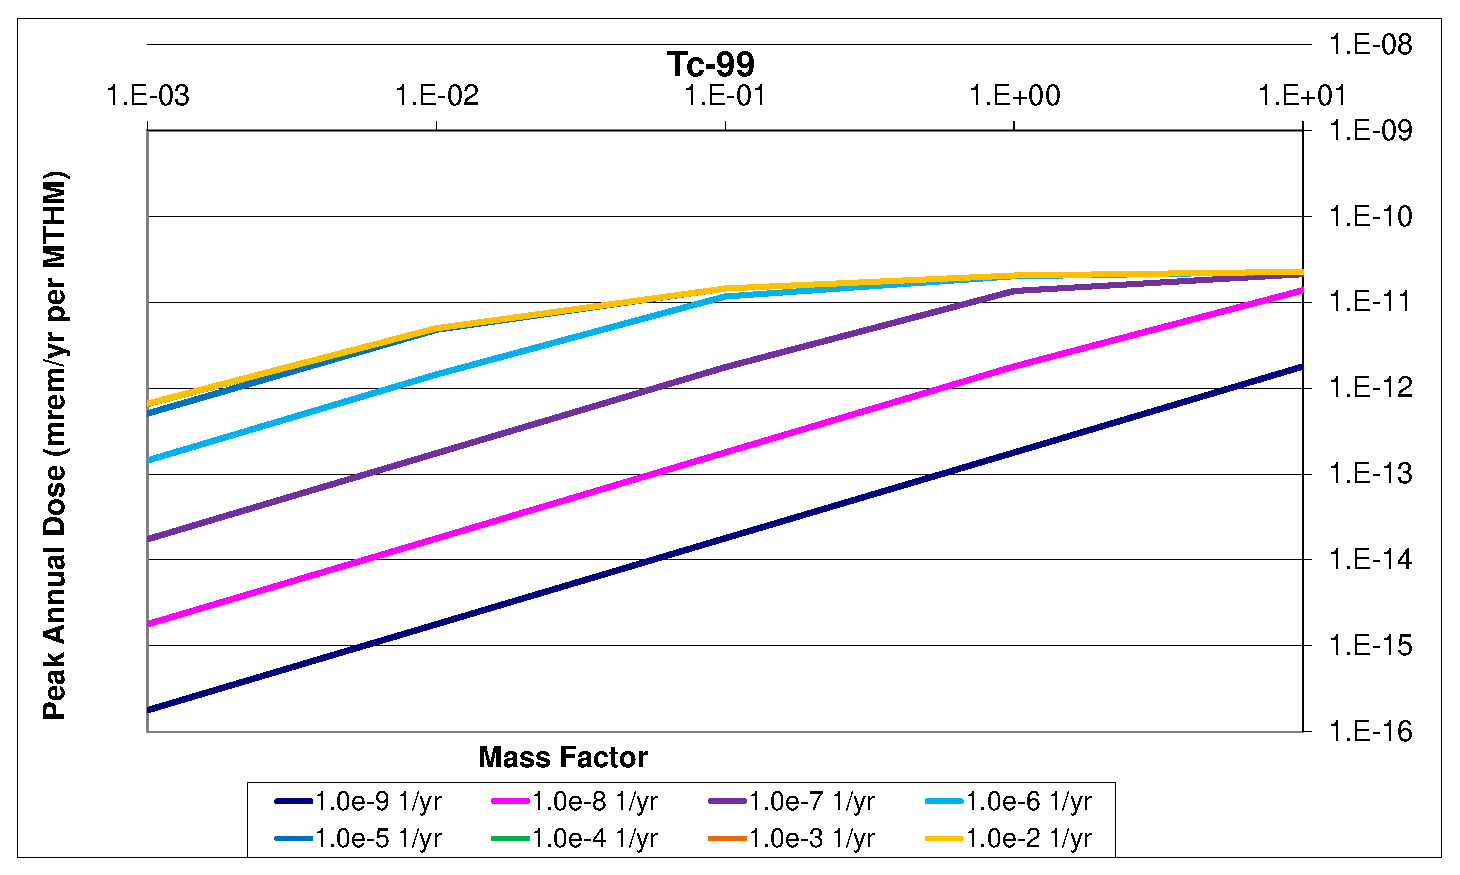
\includegraphics[width=\linewidth]{./chapters/nuclide_sensitivity/clay/WFDegAndInv/Tc-99-MF.eps}
\caption{$^{99}Tc$ inventory multiplier sensitivity.}
\label{fig:WFDegTc99MF}

\end{minipage}
\hspace{0.05\linewidth}
\hspace{0.05\linewidth}
\begin{minipage}[b]{0.45\linewidth}

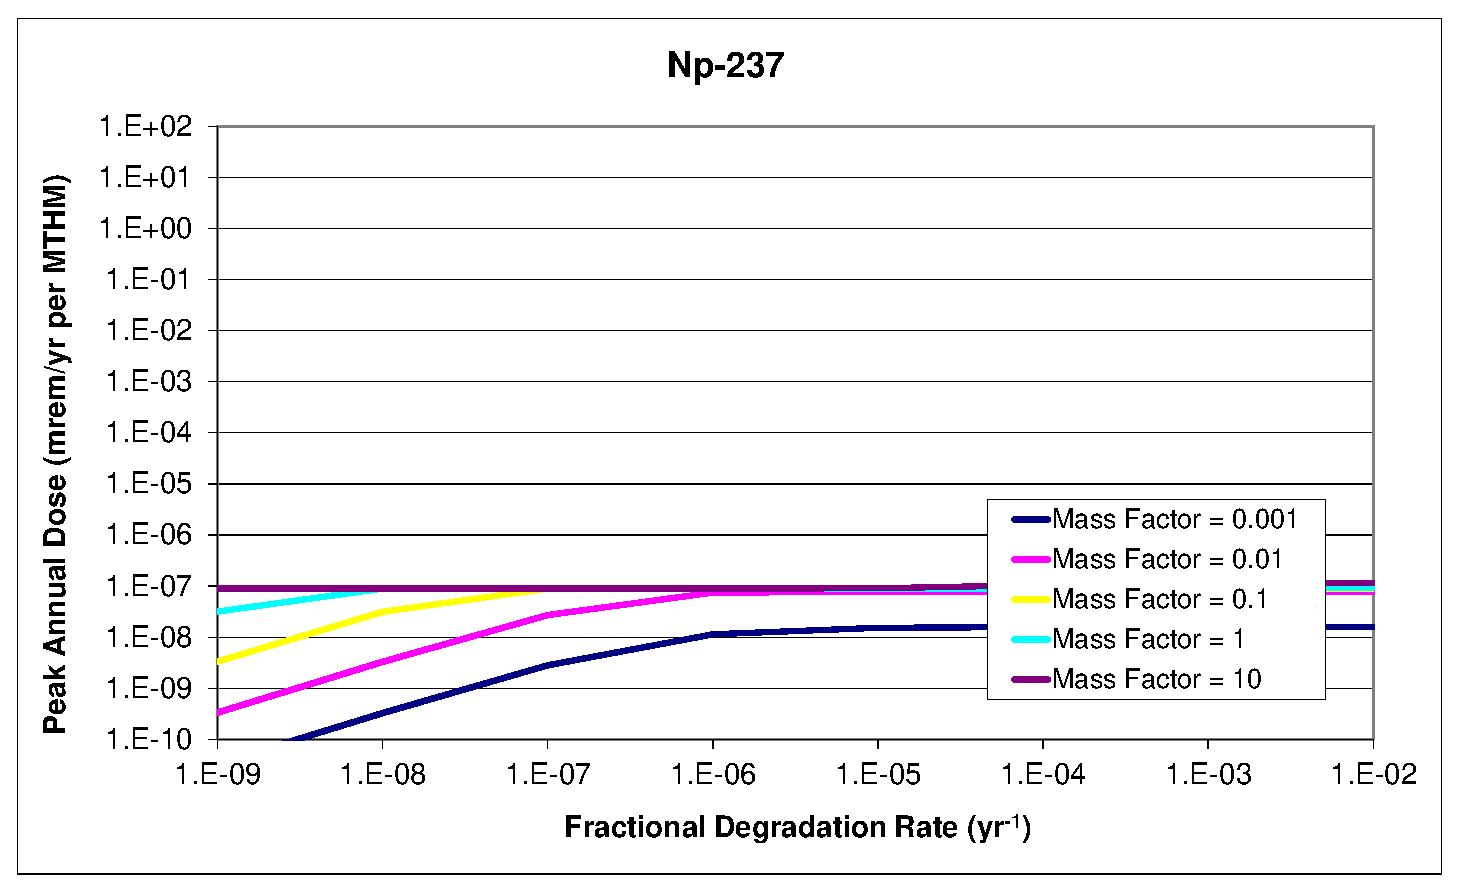
\includegraphics[width=\linewidth]{./chapters/nuclide_sensitivity/clay/WFDegAndInv/Np-237.eps}
\caption{$^{237}Np$ waste form degradation rate sensitivity.}
\label{fig:WFDegNp237}

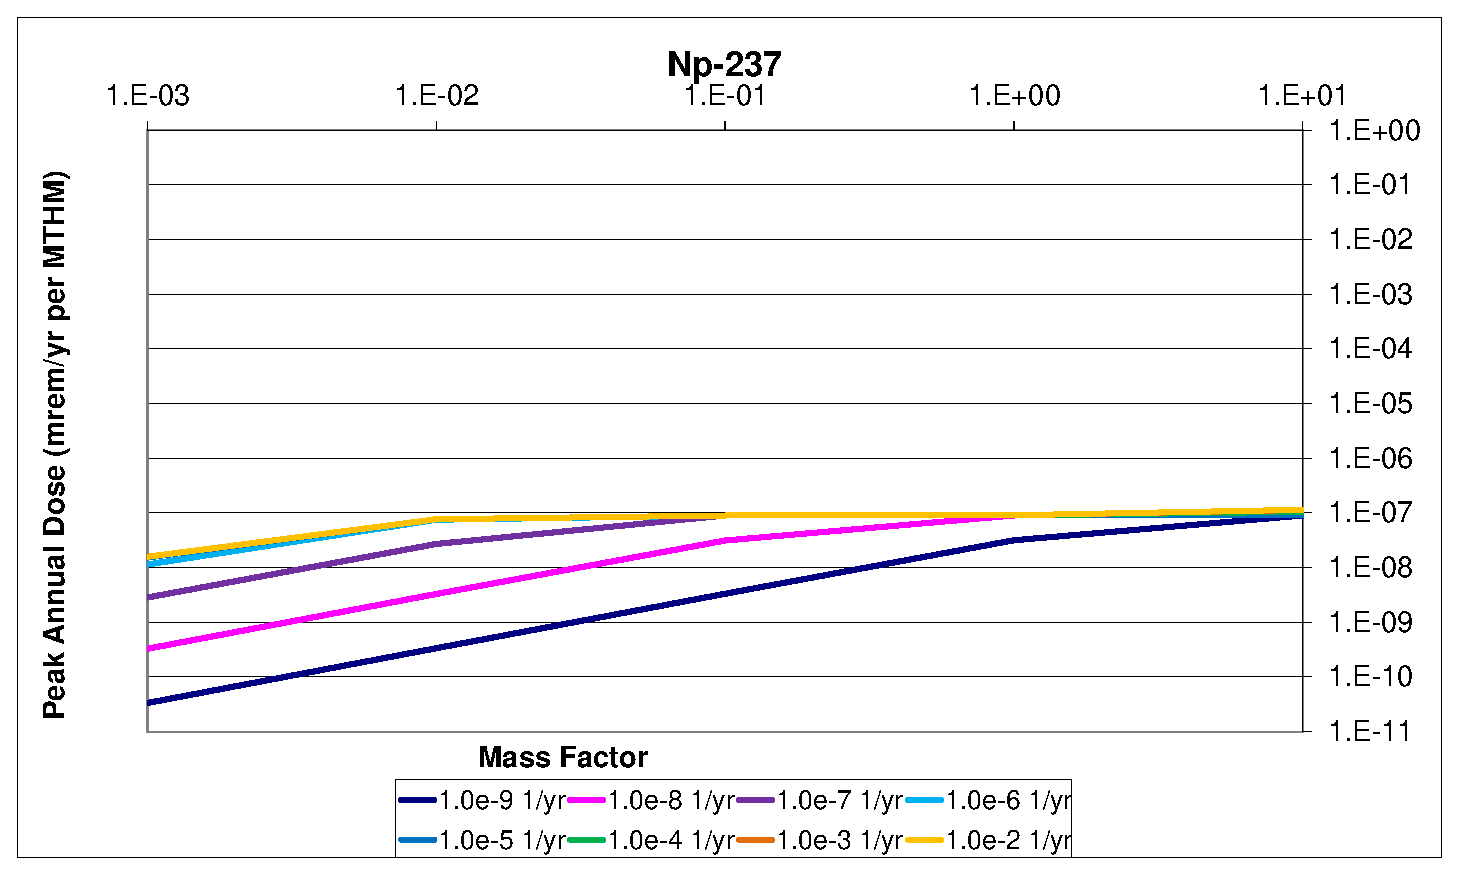
\includegraphics[width=\linewidth]{./chapters/nuclide_sensitivity/clay/WFDegAndInv/Np-237-MF.eps}
\caption{$^{237}Np$ inventory multiplier sensitivity.}
\label{fig:WFDegNp237MF}

\end{minipage}
\end{figure}
\clearpage 
